% arara: indent: {overwrite: yes}
\documentclass[a4paper]{article}
\usepackage[utf8]{inputenc}
\usepackage[russian]{babel}
\usepackage{textcomp}
\usepackage[OT1]{fontenc}
\usepackage{amsmath}
\usepackage{amsfonts}
\usepackage{amssymb}
\usepackage{float}

\author{Kirill Tolkun}

\usepackage{csquotes}

\usepackage[14pt]{extsizes}

% настройка полей документа
\usepackage{geometry}
\geometry{
	a4paper,
	total={170mm,257mm},
	top=10mm,
	right=10mm,
	bottom=15mm,
	left=10mm
}
 
\usepackage{indentfirst}

\setcounter{section}{0}

% Нумерация фурмул относительно нумерации секций
\numberwithin{equation}{section}

% Использование картинок в документе
\usepackage{graphicx}
\graphicspath{
	{lab_1/resources/}
	{lab_2/resources/}
}
\usepackage{subcaption}

\usepackage{multicol}
\setlength{\columnsep}{0cm}

% для подсветки синтаксиса
\usepackage{listings}
\usepackage{color}

\definecolor{dkgreen}{rgb}{0,0.6,0}
\definecolor{gray}{rgb}{0.5,0.5,0.5}
\definecolor{mauve}{rgb}{0.58,0,0.82}


\lstset{frame=tb,
  language=Python,
  aboveskip=3mm,
  belowskip=3mm,
  showstringspaces=false,
  columns=flexible,
  basicstyle={\small\ttfamily},
  numbers=none,
  numberstyle=\small\color{gray},
  keywordstyle=\color{blue},
  commentstyle=\color{dkgreen},
  stringstyle=\color{mauve},
  breaklines=true,
  breakatwhitespace=true,
  numbers=left,
  stepnumber=1,
  tabsize=3,
  extendedchars=\true
}

\pdfsuppresswarningpagegroup=1
\begin{document}

\begin{titlepage}
	\newpage

	\begin{center}
		МИНИСТЕРСТВО ОБРАЗОВАНИЯ РЕСПУБЛИКИ БЕЛАРУСЬ\\
		\vspace{4pt}
		БЕЛОРУССКИЙ ГОСУДАРСТВЕННЫЙ УНИВЕРСИТЕТ\\
		\vspace{4pt}
		ФАКУЛЬТЕТ ПРИКЛАДНОЙ МАТЕМАТИКИ И ИНФОРМАТИКИ\\
		\vspace{4pt}
		Кафедра технологий программирования
	\end{center}
	\vspace{12em}

	\begin{center}
		Толкун Кирилл Юрьевич
	\end{center}


	\begin{center}
		\large\textbf{Отчёт по лабораторным работам по курсу \linebreak ``Имитационное и статистическое моделирование''}
	\end{center}

	\begin{center}
		студента 4 курса 8 группы
	\end{center}

	\begin{center}
		\textbf{Вариант 10}
	\end{center}

	\vspace{5em}

	\hfill\parbox{7cm}{
		\textbf{Преподаватель:}\\
		Лобач Сергей Викторович\\
		ассистент кафедры ММАД
	}

	\vspace{2em}
	
	\begin{minipage}[t]{0.7\textwidth}
		Работа сдана \rule{2 cm}{0,2 pt} {\the\year \ г.}  \\
		\vskip 0.1em
		Зачтена \rule{2 cm}{0,2 pt} {\the\year \ г.} \\
		\vskip 0.1em
		\rule{6 cm}{0,2 pt} \\		
		\begin{small}
		\hskip 1em (подпись преподавателя)
		\end{small}
	\end{minipage}

	\vspace{\fill}

	\begin{center}
		Минск \\2020
	\end{center}

\end{titlepage}
% arara: indent: {overwrite: yes}
\section{Лабораторная 1}

\subsection{Условие}

\textbf{Согласно варианту:} $\mathbf{X_{0} = \alpha = 16 807, K = 64}$.

Используя метод Маклерена-Марсальи построить датчик БСВ (1 датчик должен быть мультипликативно конгруэнтный, второй – на выбор). Исследовать точность построенной БСВ.

\begin{enumerate}
	\item Осуществить моделирование $n = 1000$ реализаций БСВ с помощью мультипликативного конгруэнтного метода (МКМ) с параметрами $X{0}, \alpha, m = 231$;
	\item Осуществить моделирование $n = 1000$ реализаций БСВ с помощью метода Макларена-Марсальи (один датчик должен быть мультипликативно конгруэнтный (п. 1), второй – на выбор).
	      $K$ – объем вспомогательной таблицы;
	\item Проверить точность моделирования обоих датчиков (п. 1 и п. 2) с помощью критерия согласия Колмогорова и $\chi^{2}$ - критерия Пирсона с уровнем значимости $\varepsilon = 0.05$.
\end{enumerate}

\subsection{Теория}
\subsubsection{Датчики БСВ}
Для моделирования на ЭВМ реализаций \textbf{\textit{Базовой случайной величины}} используются специальные программы, называемые программными датчиками БСВ.\\
В основе программных датчиков БСВ лежат рекуррентные формулы вида:

\begin{equation}
	x_{n} = \varphi (x_{n-1}, \ldots, x_{n-p}), n = 1, 2, \ldots ,
	\label{main_recurrent:ref}
\end{equation}

где $x_{1-p}, x_{2-p}, \ldots, x_{0}$ $(p \geqslant 1)$  - заданные стартовые значения. Описанное соотношение (\ref{main_recurrent:ref}) описывает детерминированный алгоритм, однако при соответствующем подборе преобразования $\varphi(\cdot)$ получаемые на его основе псевдослучайные числа ${x_{n}}$ по своим функциональным и числовым характеристикам близки к БСВ.

Алгоритмы моделирования вида (\ref{main_recurrent:ref}) обладают общим недостатком: начиная с некоторого момента $\mathbf{t_{0}}$, последовательность псевдослучайных чисел образует цикл, который повторяется бесконечное число раз. Длина $\mathbf{T}$ циклически повторяющейся последовательности называется \textbf{\textit{периодом датчика}} БСВ $(T \leq m - 1)$.

Период $\mathbf{T}$ и \textbf{\textit{коэффициент использования}} БСВ $\mathbf{k}$ являются основными показателями качества программных датчиков БСВ. Лучшим датчикам соответствуют большие значения $\mathbf{T}$ и $\mathbf{k}$.

\subsubsection {Линейный конгруэнтный метод}\label{linear_congruential_generator}
\textbf{Линейный конгруэнтный метод} - один из методов генерации псевдослучайных чисел. Применяется в простых случаях и не обладает криптографической стойкостью. Входит в библиотеки различных компиляторов.

Суть метода заключается в вычислении последовательности случайных чисел $X_n$ следующим образом:

\begin{equation}
	X_{n+1} = \frac{\alpha X_{n} + c) \bmod m}{m},
	\label{linear_congruential_generator_formula:ref}
\end{equation}

где:

\hfill\parbox{17.5cm}{
	$
		\left.
		\begin{array}{ccc}
			\begin{aligned}
				 & \text{1. } X_{0} \text{ - начальное значение } (0 \leqslant X_{0} < 1) \\
				 & \text{2. } \alpha \text{ - множитель } (0 \leqslant \alpha < m)        \\
				 & \text{3. } c \text{ - приращение } (0 \leqslant c < m )                \\
				 & \text{4. } m \geq 2 \text{ - модуль }                                  \\
			\end{aligned}
		\end{array}
		\right\}
	$ - \textbf{\textit{параметры датчика}}.
}\\\\

\textbf{Типовые значения параметров:} $m = 2^{31}, x_0 = \alpha = 65539$.

\subsubsection{Мультипликативный конгруэнтный метод}
Метод генерации \textit{линейной конгруэнтной последовательности} (раздел \ref{linear_congruential_generator}) при $\mathbf{c = 0}$ называют \textbf{\textit{мультипликативным конгруэнтным методом}}.

\subsubsection{Метод Макларена-Марсальи}
\textbf{\textit{Генератор Макларена-Марсальи}} - криптографически стойкий генератор псевдослучайных чисел, который основан на комбинации двух конгруэнтных генераторов и вспомогательной матрице, с помощью которой происходит перемешивание двух последовательностей, полученных от двух генераторов.

Данный генератор псевдослучайных чисел оперирует с тремя объектами: двумя конгруэнтными генераторами, которые порождают последовательности $\mathbf{\langle X_n \rangle, \langle Y_n \rangle}$, и массива $\mathbf{V}$, состоящей из $\mathbf{k}$ элементов, обычно $k \in \lbrace 64, 28, 256 \rbrace$. На выходе последовательность $\mathbf{\langle Z_n \rangle}$.

Генератор состоит из четырёх основных стадий:
\begin{enumerate}
	\item Инициализация $\mathbf{V}$ и $\mathbf{Z}$ первыми $\mathbf{k}$ элементами последовательности $\mathbf{\langle X_n \rangle}$ - выполняется один раз;
	\item Выборка $\mathbf{X, Y}$ из $\mathbf{\langle X_n \rangle, \langle Y_n \rangle}$, то есть $\mathbf{X, Y}$ - очередные члены последовательностей $\mathbf{\langle X_n \rangle, \langle Y_n \rangle}$;
	\item Вычисление $\mathbf{j = \lfloor k \cdot Y \rfloor}$, где $\mathbf{j \in [0,k)}$ - случайное число, определяемое $Y$;
	\item Присвоение $\mathbf{Z_i=V_i}$ и замена $\mathbf{V_j = X}$.
\end{enumerate}

Последние три стадии могут повторяться необходимое число раз.

Данный метод позволяет ослабить зависимость между членами последовательности $\mathbf{Z_n}$ и получить сколь угодно большие значения её периода $T$ при условии, что периоды $T_1, T_2$ исходных датчиков являются взаимно простыми числами. Коэффициент использования БСВ для данного датчика $\mathbf{k=\frac{1}{2}}$ (за исключением первой реализации, для моделирования которой используется $K+1$ реализация).

\subsubsection{$\chi^2$ критерий согласия Пирсона}
\textbf{\textit{Критерий согласия Пирсона}} - это непараметрический метод, который позволяет оценить значимость различий между фактическим (выявленным в результате исследования) количеством исходов или качественных характеристик выборки, попадающих в каждую категорию, и теоретическим количеством, которое можно ожидать в изучаемых группах при справедливости нулевой гипотезы. Метод позволяет оценить статистическую значимость различий двух или нескольких относительных показателей (частот, долей).

Данный критерий применяют для проверки гипотезы о соответствии эмпирического распределения предполагаемому теоретическому распределению $F(X)$ при большом объёме выборки $(n \geqslant 100)$. \textit{Критерий применим для любых видов функции $F(x)$, даже при неизвестных значениях их параметров, что обычно имеет место при анализе результатов механических испытаний}.\\

Статистика критерия проверки гипотез имеет вид:

\begin{equation}
	\chi^{2} = \sum_{i=1}^{p} \frac{(n_{i} - n \cdot p_{i})^{2}}{n \cdot p_{i}},
\end{equation}

где $n_{i}$ - наблюдаемые частоты, $n \cdot p_{i}$ - ожидаемые частоты.\\

Чем больше $\chi^{2}$, тем сильнее выборка $X$ не согласуется с гипотезой $H_0$ (\textbf{\textit{нулевая гипотеза}}: наблюдаемые частоты соответствуют ожидаемым).

Чтобы проверить гипотезу по \textit{критерию Пирсона} необходимо сравнить \textit{статистику критерия} с \textit{критическим значения}, которой находится в таблице для соответствующего \textit{уровня значимости} и количеству \textit{степеней свободы}.\\

\textbf{Пример:}
при уровне значимости $\alpha = 0.05$ и количестве степеней свободы $\nu = 9$ \textit{критерий Пирсона} согласуется с \textit{нулевой гипотезой} при $\chi^{2} < 16.919$.

\begin{figure}[h!]
	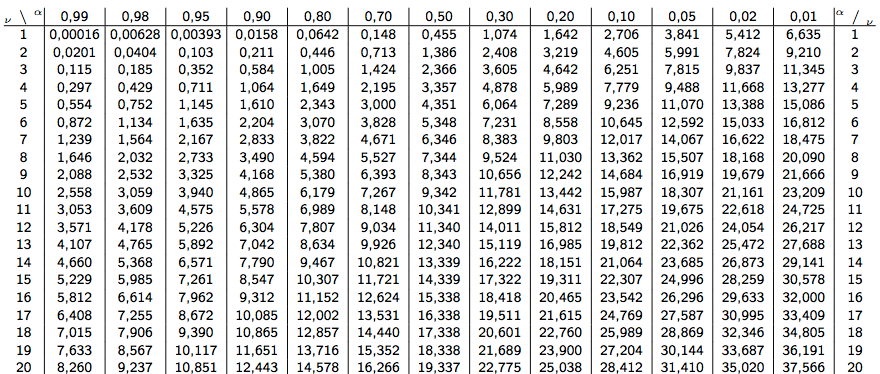
\includegraphics [width=\textwidth] {pirson_critical_values.png}
	\caption{Значения $\chi^2$ при различных $P_{\chi^{2}}$ в зависимости от числа степеней свобод $\nu$.}
	\label{fig:pirson_critical_values}
\end{figure}

\subsubsection{Критерий согласия Колмогорова}
\textbf{\textit{Критерий согласия Колмогорова}} предназначен для проверки гипотезы о принадлежности выборки некоторому закону распределения, то есть проверки того, что эмпирическое распределение соответствует предполагаемой модели.

\textbf{\textit{Эмпирическая функция распределения}} $\mathbf{F_{n}}$, построенная по выборке $X = (X_{1}, \ldots, X_{n})$, имеет вид:
\begin{equation}
	F_{n}(x) = \frac{1}{n} \sum_{i=1}^{n}I_{X_{i} \leqslant x}
\end{equation}

где $I_{X_{i} \leqslant x}$ указывает, попало ли наблюдение $X_{i}$ в область $(-\infty, x]$:
\begin{equation}
	I_{X_{i} \leqslant x} =
	\begin{cases}{}
		1, X_{i} \leqslant x \\
		0, X_{i} > x         \\
	\end{cases}
\end{equation}

\textbf{\textit{Статистика критерия}} для эмпирической функции распределения $F_{n}(x)$ определяется следующим образом:
\begin{equation}
	D_{n} = \sup_{x \in R} |F_{n}(x) - F(x)|
\end{equation}

\textbf{Принятие решения по критерию Колмогорова:}
В случае справедливости \textit{нулевой гипотезы} ($H_{0}$) при $n \rightarrow + \infty$ статистика $D_{n}$ имеет распределение Колмогорова:
\begin{equation}
	\lim_{n \rightarrow \infty} P(\sqrt{n} D_{n} < x) = K(x)
\end{equation}
здесь
\begin{equation}
	K(x) = \sum_{k = -\infty}^{+\infty} (-1)^{k} e^{-2k^{2}x^{2}} \approx 1 - 2e^{-2x^{2}}, x \geqslant 0
	\label{kolmogorov_distribution_function}
\end{equation}
- функция Колмогорова.\\

При \textbf{\textit{уровне значимости}} $\alpha$ пороговое значение $C_{\alpha}$, находится из соотношения:
\begin{equation}
	K(C_{\alpha}) = 1 - \alpha
	\label{threshold_value}
\end{equation}

Таким образом, для проверки гипотезы о виде распределения получаем:

\begin{equation}
	\rho (X) =
	\begin{cases}{}
		H_{0}, если \sqrt{n} D_{n} \leqslant \alpha, \\
		H_{1}, если \sqrt{n} D_{n} > \alpha.         \\
	\end{cases}
\end{equation}

\begin{figure}[t!]
	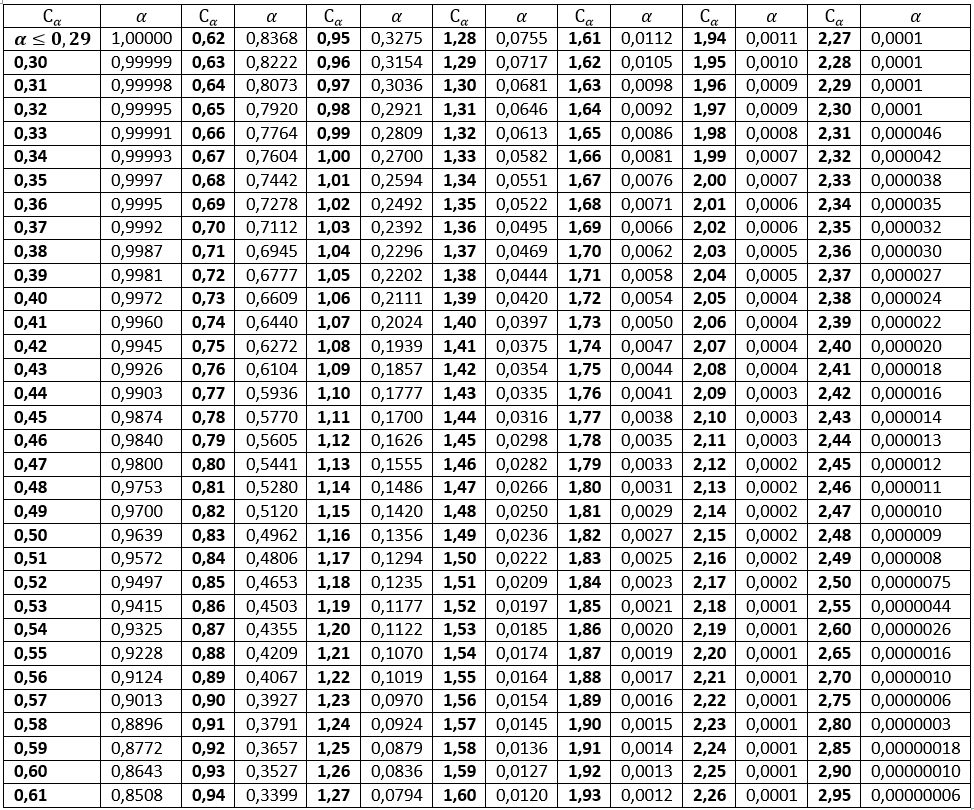
\includegraphics [width=\textwidth] {kolmogorov_critical_values.png}
	\caption{Значения $C_{\alpha}$ при различных $\alpha$.}
	\label{fig:pirson_critical_values}
\end{figure}

\newpage
\textbf{Пример:}
при уровне значимости $\alpha = 0.05$ и пороговое значение из соотношений (\ref{kolmogorov_distribution_function}), (\ref{threshold_value}) $\mathbf{C_{\alpha} \approx 1.359}$.\\

\textbf{Критерий согласия Колмогорова для непрерывного равномерное распределения}\\

\textbf{\textit{Непрерывное равномерное распределение}} - распределение случайной вещественной величины, принимающей значения, принадлежащие некоторому промежутку конечно длины, характеризующая тем, что плотность вероятности на этом промежутке почти всюду постоянна.

\textbf{\textit{Функция распределения:}}
\begin{equation}
	F_{X}(x)\equiv P(X \leqslant x) =
	\begin{cases}{}
		0, x < a                           \\
		\frac{x-a}{b-a}, a \leqslant x < b \\
		1, x \geqslant b                   \\
	\end{cases}
\end{equation}

\textbf{\textit{Значения теоретическая функция распределения}} для интервала $[0, 10$:
\begin{equation}
	F(x) = \frac{x - 0}{1 - 0} = x
\end{equation}

\textbf{\textit{Значения эмпирической функции распределения}}.

Для $x_{i}$ из выборки $X$, значение эмпирической функции распределения:
\begin{equation}
	F_{n}(x) = \frac{n_{i}}{n}
\end{equation}

где $n$ - количество элементов в выборке, $n_{i}$ - количество элементов в выборке меньших $x_{i}$.

\newpage
% arara: indent: {overwrite: yes}
\section{Лабораторная 2}

\subsection{Условие}

\textbf{Согласно варианту 10:}
\begin{enumerate}
	\item Пуассона – $\Pi(\lambda), \lambda = 0.7$; Геометрическое – $G(p), p = 0.2$;
	\item Бернулли – $Bi(1, p), p = 0.75$; Пуассона – $\Pi(\lambda), \lambda = 1$;
\end{enumerate}

Смоделировать дискретную случайную величину. Исследовать точность моделирования.

\begin{enumerate}
	\item Осуществить моделирование $n = 1000$ реализаций СВ из заданных дискретных распределений;
	\item Вывести на экран несмещённые оценки математического ожидания и дисперсии, сравнить их с истинными значениями;
	\item Для каждой из случайных величин построить свой $\chi^{2}$-критерий Пирсона с уровнем значимости $\varepsilon = 0.05$. Проверить, что вероятность ошибки I рода стремится к 0.05;
	\item Осуществить проверку каждой из сгенерированных выборок каждым из построенных критериев.
\end{enumerate}

\subsection{Теория}
\subsubsection{Датчик случайной величины распределения Пуассона}

\textbf{Распределение Пуассона} -  распределение дискретного типа случайной величины, представляющей собой число событий, произошедших за фиксированное время, при условии, что данные события происходят с некоторой фиксированной средней интенсивностью и независимо друг от друга.\\

\textbf{Функция распределения:}
\begin{equation}
	\frac{\Gamma (k+1,\lambda)}{k!}.
\end{equation}

\textbf{Функция вероятности:}
\begin{equation}
	\frac{e^{-\lambda}\lambda^{k}}{k!}.
\end{equation}

\textbf{Математическое ожидание:} $\lambda$.\\

\textbf{Дисперсия:} $\lambda$.

\paragraph{Алгоритм моделирования:}\
\\

При моделировании будем использовать свойство пуассоновского процесса, состоящего в том, что
время ожидания появления события имеет показательное распределение:

\begin{equation}
	F_{\tau}(t) = 1 - e^{-\lambda t}.
\end{equation}

Следовательно, последовательность наступления событий в пуассоновском процессе можно задать через \textit{последовательность времён ожидания} этих событий. При этом надо проверять, чтобы суммарное время \textit{суммарное время ожидания событий в цепочке не превышала единицы}.

Последовательность времён ожидания можно получить методом обратных функций:

\begin{equation}
	\tau_{i} = - \frac{1}{\lambda} \cdot \ln(1-u_{i}),
	\label{pre_poisson_generator:ref}
\end{equation}

где $u_{i} = rnd(1)$ - \textit{случайные числа}, т.е. значения случайной величины (СВ), равномерно распределённой на [0, 1].

Последовательность (\ref{pre_poisson_generator:ref}) следует продолжать, пока не нарушается условие:

\begin{equation}
	\sum_{i=1}^{j}\tau_{i} = \sum_{i=1}^{j}(-\frac{1}{\lambda} \cdot \ln(1-u_{i} \leqslant 1.
	\label{pre_poisson_condition:ref}
\end{equation}

Максимально возможное количество слагаемых в сумме (\ref{pre_poisson_condition:ref}) и будет равно числу появления событий в данной серии, т.е. эти числа и есть значения случайной величины, имеющей распределение Пуассона.

\begin{enumerate}
	\item Во-первых, в (\ref{pre_poisson_condition:ref}) заменим выражение $1-u_{i}$ просто на $u_{i}$, поскольку они имеют один и тот же закон распределения;
	\item Во-вторых, избавимся от операций логарифмирования в каждом слагаемом, для чего пропотенциируем выражение (\ref{pre_poisson_condition:ref}).
\end{enumerate}

Таким образом, определим случайную величину:
\begin{equation}
	\xi = max \left\lbrace j : \prod_{i}^{j} u_{i} \geqslant e^{-\lambda} \right\rbrace, \lambda > 0,
\end{equation}

которая описывается распределением Пуассона. Элемент выборки можно получить последовательно увеличивая число членов $(j)$ в произведении до тех пор, пока не нарушится условие:

\begin{equation}
	\prod_{i}^{j} u_{i} \geqslant e^{-\lambda},
\end{equation}

максимальное значение $(j)$, удовлетворяющее этому условию и есть очередное значение случайной величины.\\


\textbf{\textit{Программа создания выборки:}}
\begin{figure}[h!]
	
\includegraphics [width=\textwidth] {pseudo_algorithm_poisson_generator.png}
	\caption{Псевдоалгоритм генерации СВ распределения Пуассона.}
	\label{fig:pirson_critical_values}
\end{figure}

\subsubsection{Датчик случайной величины геометрического распределения}

Под \textbf{Геометрическим распределением} в теории вероятностей подразумевают одно из двух распределений дискретной случайной величины:\

\begin{itemize}
	\item распределение вероятностей случайной величины $X$ равное номеру первого ``успеха'' в серии испытания Бернулли и принимающей значения $n = 1,2,3,\ldots$;
	\item распределение вероятностей случайной величины $Y = X - 1$, равное количеству ``неудач'' до первого ``успеха'' и принимающей значения $n = 0,1,2,\ldots$.
\end{itemize}

\textbf{Функция распределения:}
\begin{equation}
	1 - q^{n+1}.
\end{equation}

\textbf{Функция вероятности:}
\begin{equation}
	q^{n}p.
\end{equation}

\textbf{Математическое ожидание:}
\begin{equation}
	\frac{q}{p}.
\end{equation}

\textbf{Дисперсия:}
\begin{equation}
	\frac{q}{p^{2}}.
\end{equation}

\paragraph{Алгоритм моделирования:}\
\

\begin{enumerate}
	\item Моделирование реализации $\alpha$ БСВ;
	\item Принятие решения о том, что реализация $\xi$ является значением $x$, определяемым соотношением:
	      \begin{equation}
		      x = \left[ \frac{\ln \alpha}{\ln q} \right],
	      \end{equation}
	      где $[z]$ - округление числа $z$ в большую сторону до ближайшего целого значения.
\end{enumerate}

\subsubsection{Датчик случайной величины распределения Бернулли}

\textbf{Распределение Бернулли} - дискретное распределение вероятностей, моделирующее случайный эксперимент произвольной природы, при заранее известной вероятности успеха или неудачи.:\

\textbf{Функция распределения:}
\begin{equation}
	\begin{cases}{}
		0, k < 0             \\
		q, 0 \leqslant k < 1 \\
		1, k \geqslant 1     \\
	\end{cases}.
\end{equation}

\textbf{Функция вероятности:}
\begin{equation}
	\begin{cases}{}
		q, k = 0 \\
		p, k = 1 \\
	\end{cases}.
\end{equation}

\textbf{Математическое ожидание:}
\begin{equation}
	p.
\end{equation}

\textbf{Дисперсия:}
\begin{equation}
	pq.
\end{equation}

\paragraph{Алгоритм моделирования:}\
\

\begin{enumerate}
	\item Моделирование реализации $\alpha$ БСВ;
	\item Принятие решения о том, что реализация $\xi$ является значением $x$, определяемым по правилу:
	      \begin{equation}
		      x =
		      \begin{cases}{}
			      1, \alpha \leqslant p \\
			      0, \alpha > p         \\
		      \end{cases}.
	      \end{equation}
\end{enumerate}

\subsection{Код программы}

\lstinputlisting[language=Python]{./lab_2/lab2.py}

\subsection{Результат выполнения}

\begin{figure}[H]
	\centering
	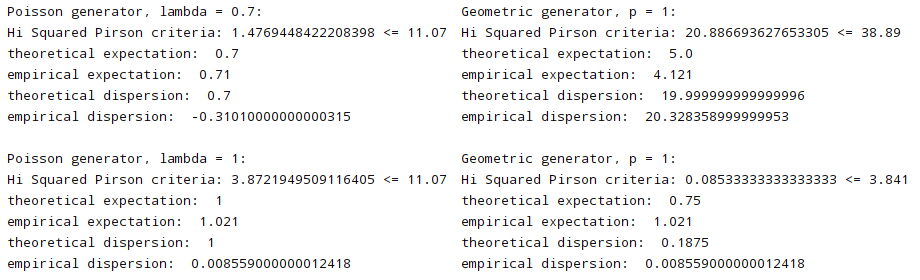
\includegraphics [width=\textwidth] {results_lab_2.jpg}
	\label{fig:results_lab_2}
	\caption{Результат выполнения программы: проверка критерием согласия Пирсона и подсчёт несмещённых оценок математического ожидания и дисперсии.}
\end{figure}

\begin{figure}[!h]
	\centering
	\begin{subfigure}[b]{0.45\textwidth}
		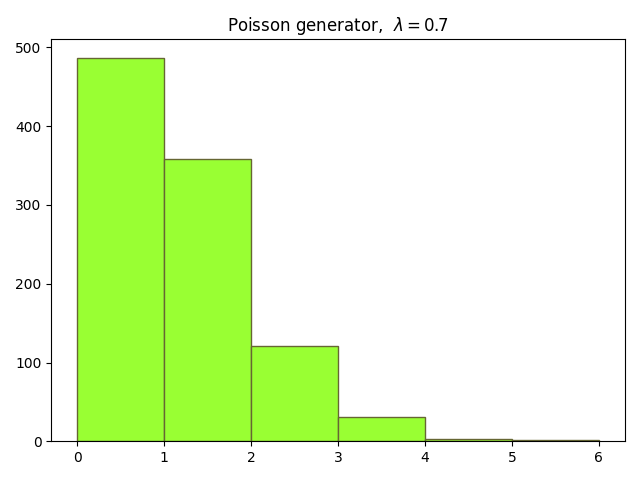
\includegraphics[width=\textwidth]{poisson_generator_l07.png}
		\caption{Диаграмма выборки, полученной генератором распределения Пуассона при $\lambda = 0.7$.}
	\end{subfigure}
	\hfill
	\begin{subfigure}[b]{0.45\textwidth}
		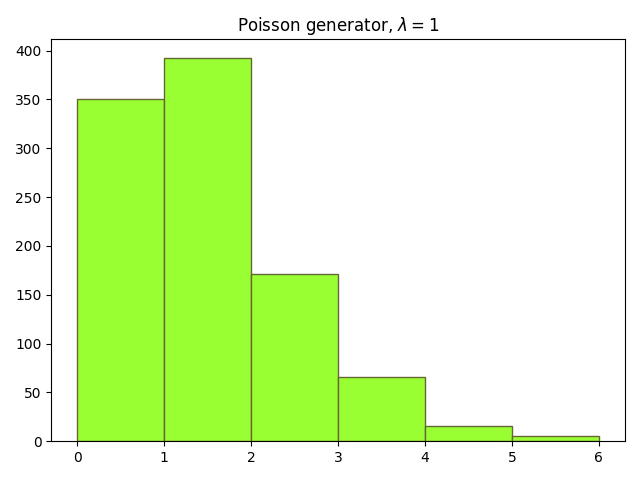
\includegraphics[width=\textwidth]{poisson_generator_l1.png}
		\caption{Диаграмма выборки, полученной генератором распределения Пуассона при $\lambda = 1$.}
	\end{subfigure}
	\\
	\begin{subfigure}[b]{0.45\textwidth}
		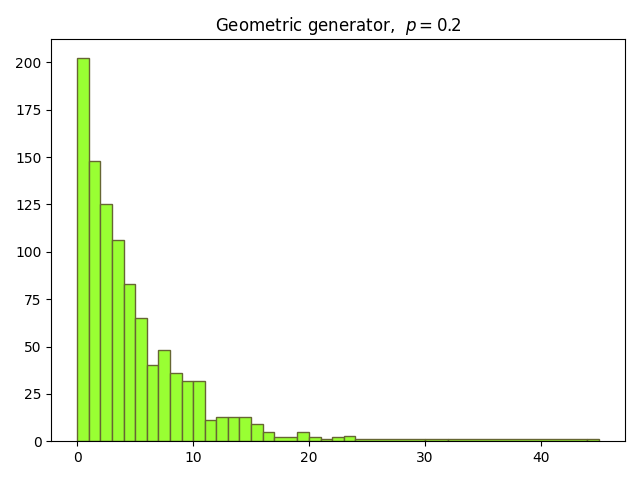
\includegraphics[width=\textwidth]{geometric_generator.png}
		\caption{Диаграмма выборки, полученной генератором геометрического распределения.}
	\end{subfigure}
	\hfill
	\begin{subfigure}[b]{0.45\textwidth}
		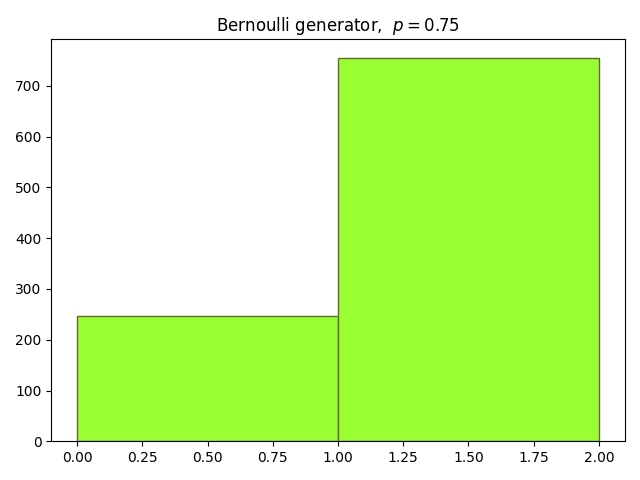
\includegraphics[width=\textwidth]{bernoulli_generator.png}
		\caption{Диаграмма выборки, полученной генератором распределения Бернулли.}
	\end{subfigure}
\end{figure}


\end{document}
